\documentclass[handout, 10pt]{beamer}

%\usepackage[backend=bibtex,firstinits=true,style=verbose-inote,citestyle=authortitle]{biblatex}
\usepackage{bm}
\usepackage{graphicx}
\usepackage{subcaption}
\usepackage{amsmath}
\usepackage{amsfonts}
\usepackage{makecell}
\usepackage{filecontents}
\usepackage{biblatex}
\usepackage{xcolor}
\usepackage{subcaption}
 \newcommand{\expect}[2][]{
\ifthenelse{\equal{#1}{}}{
\mathbb{E}\left[#2\right]
}{
\underset{#1}{\mathbb{E}}\left[#2\right]
}}

\newcommand{\cov}[2][]{
\ifthenelse{\equal{#1}{}}{
\text{Cov}\left[#2\right]
}{
\underset{#1}{\text{Cov}}\left[#2\right]
}}


\newcommand{\var}[2][]{
\ifthenelse{\equal{#1}{}}{
\text{Var}[#2]
}{
\underset{#1}{\text{Var}}[#2]
}}

\newcommand{\loss}[2][]{
\ifthenelse{\equal{#1}{}}{
\mathcal{L}(#2)
}{
\mathcal{L}_{#1}(#2)
}}

\newcommand{\kl}[2]{
\text{D}_\text{KL}[#1 \parallel #2]
}

\newcommand{\R}{\mathbb{R}}
%\newcommand{\Prob}{\mathbb{P}}

\newcommand{\1}[1]{\mathds{1}\{#1\}}


%\usecolortheme{dolphin}
\setbeamertemplate{navigation symbols}{}
\setbeamertemplate{section in toc}{\inserttocsectionnumber.~\inserttocsection}

\begin{filecontents*}{references.bib}
@InProceedings{fr_norm,
author = {Singh, Saurabh and Krishnan, Shankar},
title = {Filter Response Normalization Layer: Eliminating Batch Dependence in the Training of Deep Neural Networks},
booktitle = {Proceedings of the IEEE/CVF Conference on Computer Vision and Pattern Recognition (CVPR)},
month = {June},
year = {2020}
}
\end{filecontents*}

\addbibresource{references.bib}


\title{Filter Response Normalization Layer: Eliminating Batch Dependence in the Training of Deep Neural Networks\footnote{\citepaper{fr_norm}}}
%\subtitle{}
%\author{Ivan Skorokhodov}
%\date{}
%\logo{
\includegraphics[height=1cm]{images/ipavlov-logo.png}}

\newcommand{\citepaper}[1]{\citetitle{#1} by \citeauthor{#1}, \citeyear{#1}}

%\graphicspath{{./images}}

%\usetheme{lucid}
\begin{document}

\begin{frame}
    \titlepage
\end{frame}


\begin{frame}{Overview}
\begin{itemize}
    \item\pause BatchNorm performance degrades heavily when batch size is small
    \item\pause A lot of other normalization techniques have been proposed (LayerNorm, GroupNorm, etc), but they are insufficient
    \item\pause Authors propose two things:
    \begin{itemize}
        \item\pause \textit{Filter Response Normalization}:
\begin{equation}
y_{i}=\gamma \frac{x_{i}}{\sqrt{\nu^{2}+\epsilon}}+\beta, \qquad\text{where } \nu^{2}=\sum_{i} x_{i}^{2} / N
\end{equation}
        \item\pause \textit{Thresholded Linear Unit}
        \begin{equation}
z_{i}=\max \left(y_{i}, \tau\right)
\end{equation}
    \end{itemize}
    \item\pause These two techniques work the best when used in combination
    \item\pause Authors demonstrate superior performance for different batch sizes (from small to large ones) on ImageNet classification and MS-COCO object detection over other normalization methods
\end{itemize}
\end{frame}


\begin{frame}{Filter Response Normalization (FRN)}
\pause
We compute the norm across spatial locations and normalize the input with it:
\begin{equation}
y_{i}=\gamma \frac{x_{i}}{\sqrt{\nu^{2}+\epsilon}}+\beta, \qquad\text{where } \nu^{2}=\sum_{i} x_{i}^{2} / N
\end{equation}

\pause
A problem with FRN occurs when $N = H \times W$ is too small: in this case small values of $\epsilon$ diverge the procedure into a sign function:
\begin{figure}
\centering
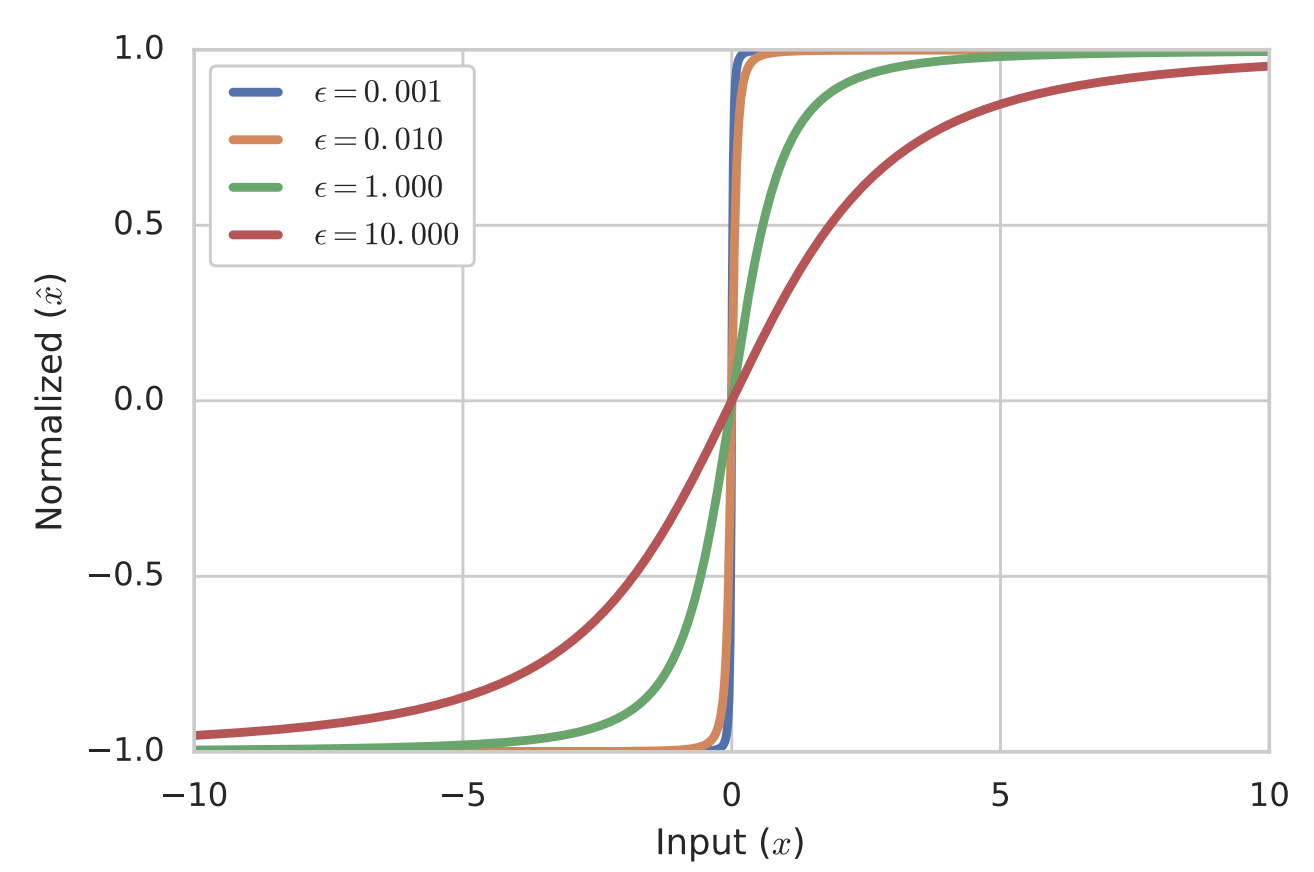
\includegraphics[width=0.5\textwidth]{images/sign-function-divergence}
\end{figure}

That's why authors initialize $\epsilon = 0.0001$ for $N=1$ and learn it.
\end{frame}


\begin{frame}{Thresholded Linear Unit (TLU)}
\begin{itemize}
    \item\pause One of the main differences between FRN and BN is that FRN does not keep activations zero-centered (by subtracting the mean)
    \item\pause This may make them deviate arbitrarily far away from zero 
    \item\pause And this consequently pushes ReLU into bad zones (all-zeros or all-linear)
    \item\pause That's why authors turn ReLU activation into TLU:
\begin{equation}
\boldsymbol{z}=\max (\boldsymbol{y}, \tau)
\end{equation}
where $\tau$ is a learnable bias.
\item\pause In practice, it showed to perform well
\end{itemize}
\end{frame}


\begin{frame}{Classification results on ImageNet}
\begin{figure}
\centering
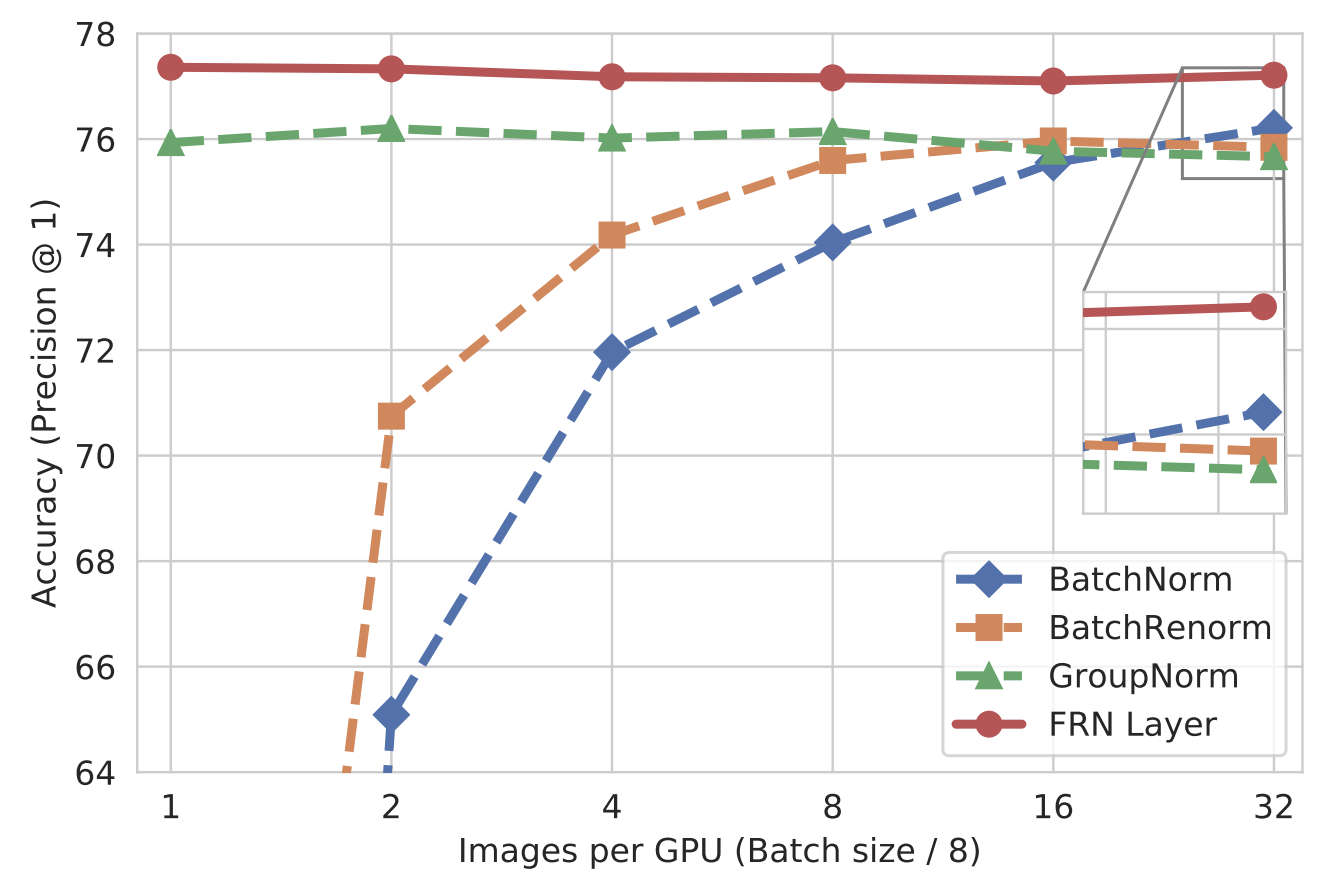
\includegraphics[width=0.8\textwidth]{images/imagenet-results}
\caption{ImageNet results for ResNetV2-50}
\end{figure}
\end{frame}


\begin{frame}{MS-COCO object detection results}
\begin{figure}
\centering
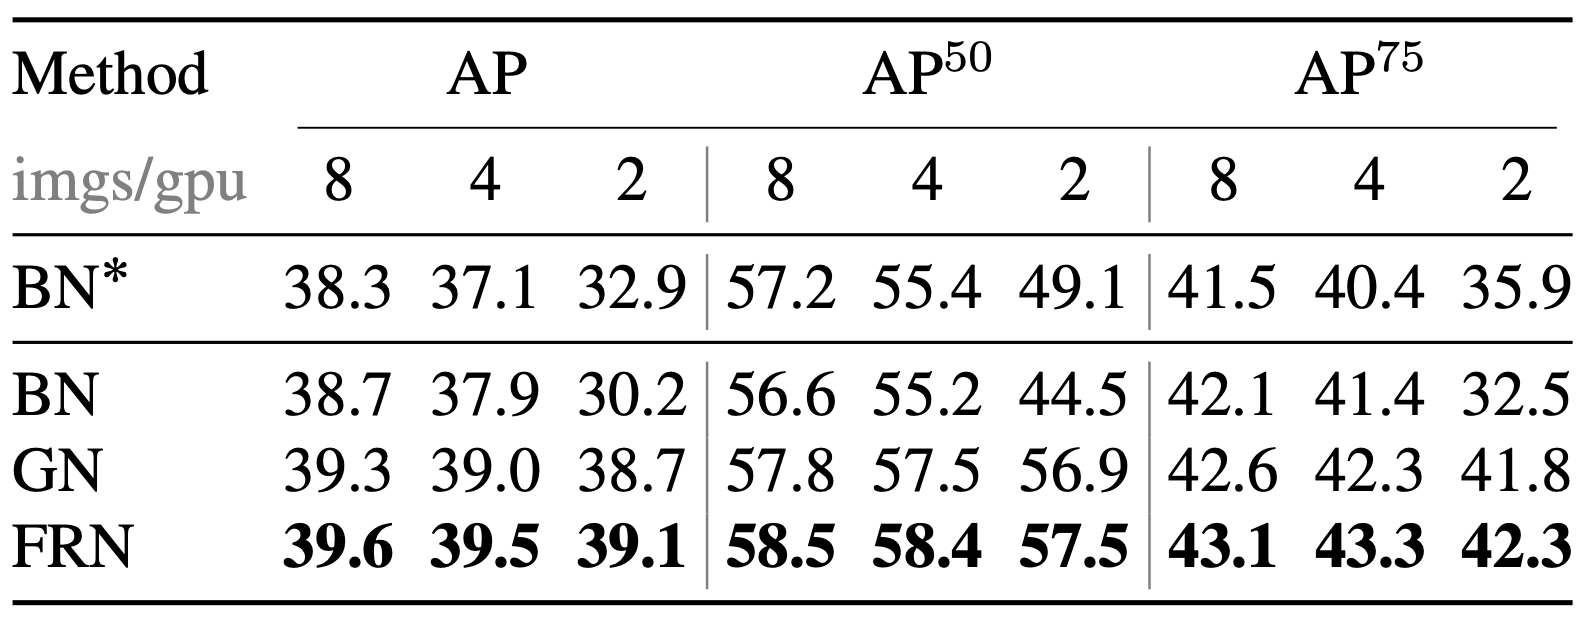
\includegraphics[width=0.5\textwidth]{images/object-detection-results}
\caption{RetinaNet with Resnet101 FPN backbone}
\end{figure}
\end{frame}


\begin{frame}{FRN/TLU ablation}
\begin{figure}
\centering
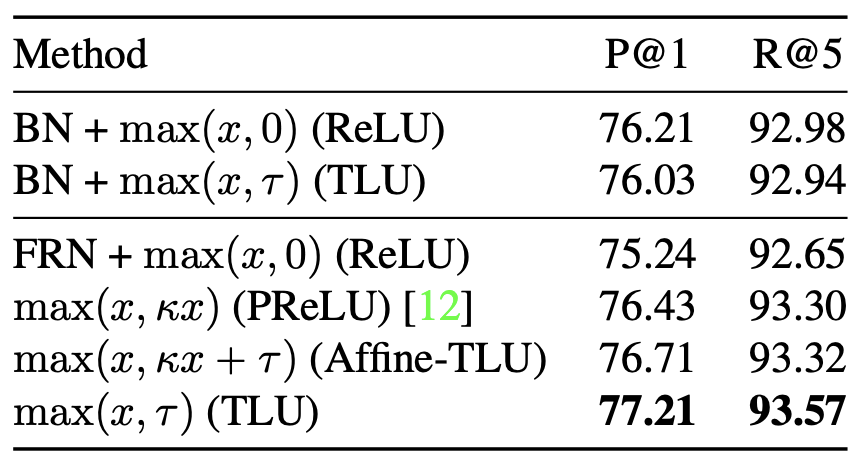
\includegraphics[width=0.5\textwidth]{images/frn-tlu-ablation.png}
\caption{Results for difference normalization/activation setups for ImageNet classification}
\end{figure}
\end{frame}


\begin{frame}{Final thoughts}
\begin{itemize}
    \item\pause Other normalization techniques (LN, GN, etc) work better than BN on small batch sizes, but worse on large ones
    \item\pause Authors managed to ``take the best of the both worlds'' 
    \item\pause Authors argue that LN/GN perform poorly because they create additional correlations between channels
    \begin{itemize}
        \item\pause That's an interesting perspective
    \end{itemize}
    \item\pause It's interesting to see that parameters $\epsilon$ and $\tau$ are learnt to meaningful values
    \begin{itemize}
        \item\pause Usually such kind of parameters are not optimized well
    \end{itemize}
\end{itemize}
\end{frame}


\end{document}
